\documentclass[a4paper,14pt]{extreport}
\usepackage[utf8]{inputenc}
\usepackage[russian]{babel}
\usepackage{titlesec}
\usepackage{titletoc}
\usepackage{appendix}
\usepackage{graphicx}
\usepackage{indentfirst}
\usepackage{listings}
\usepackage[normalem]{ulem}
\usepackage{geometry} % Меняем поля страницы
\geometry{left=3cm}% левое поле — не менее 20 мм
\geometry{right=2cm}% правое поле — не менее 10 мм
\geometry{top=2cm}% верхнее поле — не менее 15 мм
\geometry{bottom=2cm}% нижнее поле — не менее 20 мм
\renewcommand{\baselinestretch}{1.25}
\graphicspath{{images/}}
\parindent=1.25cm
\frenchspacing
\clubpenalty=10000
\widowpenalty=10000
\sloppypar
\lstset{language=python,columns=fullflexible,extendedchars=true,showstringspaces=false}
\begin{document}
\thispagestyle{empty}

\enlargethispage{2cm}
{
\begin{center}
\renewcommand{\baselinestretch}{1.25}
{
\selectfont
Министерство образования и науки Российской Федерации

Ярославский государственный университет им.~П.\,Г. Демидова

Кафедра компьютерных сетей

\vspace{6cm}

{\em Курсовая работа}


\vspace{0.5cm}

{ \Large \bf Разработка сетевой архитектуры для редактора диаграмм связей
HiveMind}

\vspace{3cm}

\hfill\parbox{7cm}
{ 
Научный руководитель

ст. преподаватель\\
\hbox to 1.5cm{\hrulefill} И.\,В.~Парамонов

<<\hbox to 0.5cm{\hrulefill}>> \hbox to 2.3cm{\hrulefill} 2011 г.
}

\vspace{1.5cm}

\hfill\parbox{7cm}
{ 
Студент группы ИВТ-42СО\\
Кандауров О.В.

<<\hbox to 0.5cm{\hrulefill}>> \hbox to 2.3cm{\hrulefill} 2011 г.
}

\vspace{5cm}

Ярославль 2011
}
\end{center}
}

\newpage
\tableofcontents
\newpage

\chapter*{Введение}
\label{chap:introduction}
\addcontentsline{toc}{chapter}{Введение}

В современном мире, почти каждый человек, живущий в развитой стране, использует
мобильные устройства в своём быту. Существует множество классов данных
устройств, таких как: мобильные телефоны, смартфоны, КПК, планшеты. Мобильные
устройства прочно вошли в жизнь человека. С каждым годом наращивается функционал
и производительность данных устройств. Многие люди находят в данных устройствах
замену своему стационарному компьютеру. Мобильные устройства оснащаются
средствами связи, такими как wi-fi, bluetooth, 3G, что позволяет обладателю
данного устройства пользоваться интернетом, взаимодействую с другими
пользователями.

Диаграммы связей --- это графическое представление данных, имеющих
иерархическую структуру. Они позволяют создавать, отображать и
структурировать некоторую иноформацию. У диаграмм связи нет ограничений на
структуру данных, за исключением иерархческого порядка, поэтому они могут
использоваться для работы с различной инофрмацией. Они успешно
применяются для генерации идей, конспектирования докладов, написания планов
статей, составление презентаций и так далее.

Диаграммы связи используются во множестве различных ситуаций связанных с работой
над данными. Зачастую работа над данными требует участия группы людей. В данной
ситуации возникает несколько проблем. Во-первых, людям, участвующим в данном
процессе необходимо собраться в одном месте, чтобы начать совместную работу.
Во-вторых, сложно предоставить всем участникам процесса равноценный доступ к
диаграмме связи, например только один человек может сидеть за компьютером, либо
писать на доске.

Решение вышеназванных проблем заключается в том, чтобы использовать возможности
мобильных устройств. Мобильные устройства портативны, что позволяет их с
легкостью всегда держать при себе. Также они оснащены средствами доступа в
интернет. Идея заключается в том, чтобы предоставить людям равные возможности по
внесению своего вклада в создание диаграмм, в любое время, в любом месте,
используя мобильное устройство или персональный компьютер.

В данной работе описывается реализация функции совместного редактирования в
редакторе диаграмм связей под названием HiveMind. Данный проект разрабатывается
с начала 2010 года группой студентов рамках программы FRUCT. HiveMind имеет
множество функций для редактирования диаграмм связей и поддержку платформ
Windows, Maemo, MeeGo, Linux. Проект направлен на достижение максимальной
мобильности пользователей, повышение производительности труда и увеличение
потенциальных решений в поставленных задачах.


\newpage

\chapter{Мотивация и постановка задачи}\label{ch:chapter_1}

\section{Диаграммы связей}
Диаграмма связей реализуется в виде древовидной схемы, пример на рис.~\ref{ris:mindmap}.
\begin{figure}[h!]
\centering
\includegraphics[width=1\linewidth]{mind-map}
\caption{Пример диаграммы связей}
\label{ris:mindmap}
\end{figure}

Возможность сворачивать узлы дает большее удобство для редактирования больших диаграмм, возможность сосредоточиться на какой то отдельной части диаграммы. Так же при различном оформлении отдельных узлов (цвет текста, цвет фона, рамка вокруг текста, применение пиктограмм), соединительных линий можно повысить более четкое разграничение различных частей диаграммы. Облака обычно применяются для выделения очень важных ключевых идей. В диаграммах связей могут быть использованы гиперссылки на веб-страницы, локальные файлы или адреса электронной почты. Так же используются графические связи, чтобы показать взаимосвязь элементов, находящихся в различных частях диаграммы. На рис. можно видеть пример применения некоторых вышеописанных атрибутов узлов.

\section{Обзор существующих редакторов диаграмм связей}\label{sec:overview_of_mind_map}

В этом разделе производится обзор существующих редакторов диаграмм связей, а так же оценка их применимости, достоинства и недостатки. Так как для некоторых платформ существует больше редакторов, чем для других, то будут рассмотрены самые популярные из них.

\subsection{Редакторы диаграмм для iPhone}

Мобильные устройства на платформе iPhone являются одними из самых распространенных в мире, для данной платформы существует очень много приложений для решения различных задач, в том числе существуют несколько приложений для редактирования диаграмм связей.

Одно из известных приложений для редактирования диаграмм связей "--- это MindNode. Данная программа имеет версии как для компьютера так и для iPhone, но компьютерная версия программы реализована только для системы Mac OS X.

MindNode имеет однопользовательский интерфейс редактирования диаграммы, с возможностью экспорта в различные форматы: формат MindNode, FreeMind, в виде изображения формата .png, древовидный список в виде простого текста, а так же в виде OPLM файла (язык разметки, основанный на XML).

Программа поддерживает работу как в вертикальном так и в горизонтальном режимах. Диаграмму можно приближать и удалять. Так же программа поддерживает поиск текста по узлам, реализована возможность изменять цвет связей, создавать/переименовывать/удалять элементы, сортировать элементы схемы.

В целом программа удобна для использования. Однако, существенный минус ее "--- это цена. Программу можно приобрести в AppStore за \$5.99. Для того чтобы иметь возможность синхронизации с компьютером, придется заплатить еще \$20.

Так же популярным редактором для платформы iPhone является редактор MindJet. У данного приложения возможностей намного больше чем у MindNode. Отличительной особенностью MindJet являются: работа с иконками, сворачивать и разворачивать ветви, функции управления задачами "--- начальная и конечная даты выполнения задачи. Цена на такую программу составляет около 6 евро.

\subsection{Редакторы диаграмм для платформы Android}

Платформа Android "--- одна из популярных платформ, основанная на ядре Linux. Платформа базируется на Dalvik virtual machine, поэтому преимущества и возможности операционной системы Linux на данной платформе практически не используются.

MindMap memo "--- известный редактор диаграмм связей для платформы Android. Он имеет скудную функциональность: масштабирование, копирование/вставка, изменение цвета узла, работа с иконками, сворачивание/разворачивание веток, изменение фона. Умеет экспортировать и импортировать файлы в формате FreeMind.

\subsection{Мультиплатформенные редакторы диаграмм}

MindMeister "--- одна из мощнейших Web 2.0 сервисов для мобильных устройств на платформах iPhone и Maemo. Ее отличительные особенности это совместная работа над диаграммой в режиме реального времени через интернет, так же возможна работа в оффлайн режиме.

Программа взаимодействует с онлайновым сервисом Mindmeister который и реализует хранение и совместную работу над диаграммами.

Из преимуществ стоит отметить очень широкий набор инструментов: иконки, изменение цветов узлов, связей, фона, чат, поиск текста, SSL. Из недостатков "--- бесплатная версия программы позволяет пользователю создавать до 3 интеллект-карт и импорт карт из FreeMind. Платные же версии стоят \$9 в месяц, либо \$59 в год.

В данном классе приложений существует крайне мало бесплатных версий. Функциональность некоторых из них очень бедны, в частности MindNode не умеет работать с иконками, под платформу Maemo 5 вообще нет приложений такого типа, более того, все рассмотренные приложения кроме MindMeister вообще не поддерживают совместное редактирование диаграмм связей.

\section{Описание проекта}\label{sec:project_summary}

Совмещение таких технологий, как мобильные устройства и диаграммы связей "--- очень перспективно, в первую очередь для повышения мобильности участников, которые работают над диаграммой. Так же это позволяет уменьшить затраты на проведение совместной работы над диаграммами связей. Но в данный момент инструментов под мобильные устройства практически нет. Поэтому было решено создать проект по разработке приложения, которое обладало бы богатой функциональностью и поддерживало режим совместного редактирования диаграмм.

Основной целью проекта является разработка редактора диаграмм связей с поддержкой совместного редактирования диаграмм связей для мобильных устройств. Редактор должен использовать формат FreeMind, для обеспечения свободного чтения и редактирования файлов, созданных как на мобильных устройствах, так и на настольных компьютерах.

Основные возможности:
\begin{itemize}
\item Чтение и запись файлов в формате FreeMind
\item Отображение диаграмм связей и навигация по ним
\begin{itemize}
\item Поддержка работы с несколькими диаграммами
\end{itemize}
\item Поддержка совместного редактирования диаграмм
\item Особенности пользовательского интерфейса
\begin{itemize}
\item Интернационализация
\item Использование клавиатуры и сенсорного дисплея
\end{itemize}
\end{itemize}

При совместной работе возникает необходимость коммуникации между членами группы. По этой причине в приложение должен быть встроен простейший сервис обмена текстовыми сообщениями.

Ввиду того, что проект предполагает полностью распределенную среду общения между устройствами, что является новым для данной категории приложений, то необходим поиск концепции эффективной модели совместного редактирования диаграмм связей.

\section{Обзор платформы Maemo 5}\label{sec:compare_platforms}

Для реализации проекта была выбрана платформа Maemo 5.
Maemo представляет собой встраиваемую ОС, разработанную на базе дистрибутивов Debian и предназначенную для устройств финской корпорации с процессорами ARM. Система основана на ядре GNU/Linux, свободно распространяемых программах, а также собственных разработках Nokia, многие из которых — закрыты. Другое важное отличие "--- Maemo не ориентирована, как Android, на Java-приложения и дает разработчикам большую свободу. В частности, на Maemo 4 были перенесены многие популярные открытые программы. Nokia выпускает и SDK для разработчиков приложений.

Архитектура системы. В нижней части программного стека располагается загрузчик NoLo (Nokia Loader), ядро GNU/Linux, которое управляет памятью, процессами, устройствами, файловой системой, осуществляет взаимодействие между процессами, а также предоставляет API программам, работающим в пространстве пользователя (т.н. userspace). В общем, все устроено как в любом другом дистрибутиве Linux, с учетом аппаратных особенностей устройств Nokia. Далее рассмотрим системные сервисы и основные библиотеки:
\begin{itemize}
\item
GLib — низкоуровневая библиотека, расширяющая возможности, стандартной библиотеки libc языка C (она служит основой для GTK+ и Gnome);
\item
D-Bus — шина сообщений, которая предоставляет приложениям широкий набор средств межпроцессного взаимодействия. Программа разрабатывается в рамках проекта freedesktop.org и активно используется во многих открытых проектах (например, в Gnome и KDE);
\item
HAL (Hardware Abstraction Layer) — демон, предоставляющий слой аппаратных абстракций. Первоначально был разработан в компании RedHat, сейчас HAL является частью все того же freedesktop.org;
X Window System — графическая подсистема, обеспечивающая возможность работы GUI-приложений.
\end{itemize}
 
На следующем уровне находятся библиотеки GTK+, а также необходимые для них средства (cairo, Pango и ATK).

На самом верхнем уровне находится среда рабочего стола Hildon, которая представляет из себя смесь компонентов Gnome, открытых разработок сообщества и собственных средств Nokia. Собственно, Hildon можно считать «мобильной» вариацией среды рабочего стола Gnome.

Недавно был анонсирован переход Maemo на графические библиотеки QT. При этом, GTK+/Hildon получит статус поддерживаемого сообществом. Понятно, что при таком серьезном изменении архитектуры следующий релиз системы не может быть развитием текущего. Тем не менее, MeeGo будет отличаться от Maemo 5 едва ли не сильнее, чем она сама — от Maemo 4. Т.е. разработка проекта уже разошлась на две независимых ветки и при всех несомненных достоинствах, Maemo 5 является не более чем переходной версией.

\section{Используемый инструментарий}\label{sec:choose_toolkit}

Nokia N900 "--- смартфон от компании Nokia, работающий под управлением операционной системы Maemo 5.
Nokia N900 является первым устройством, основанным на микропроцессоре TI OMAP3 с ядром ARM Cortex-A8.
В отличие от предыдущих интернет-планшетов компании, N900 является первым, обладающим функциями телефона.
Также аппарат работает как 5-мегапиксельная камера, портативный медиа-плеер и Интернет клиент с возможностью работы с электронной почтой и веб-браузером.
Он имеет 3.5-дюймовый резистивный сенсорный экран с разрешением 800х480 пикселей. Устройство снабжено тактильной (вибрация) и звуковой (клик) отдачей при вводе данных.
Смартфон имеет выдвижную трехстрочную подсвечиваемую клавиатуру.
В дополнение к английской QWERTY-раскладке, выдвижная клавиатура обеспечена итальянской, французской, немецкой, русской или финской/шведской раскладками.

Qt "--- кросс-платформенный инструментарий разработки ПО на языке программирования C++~\cite{qt_4, qt_4_with_examples}.
Существуют также «привязки» ко многим другим языкам программирования: Python (PyQt, PySide), Ruby (Qt-Ruby), Java (Qt Jambi), PHP (PHP-Qt) и другие.

Библиотека включает в себя все основные классы, которые могут потребоваться при разработке прикладного программного обеспечения, начиная от элементов графического интерфейса и заканчивая классами для работы с сетью, базами данных и XML. Qt является полностью объектно-ориентированным, легко расширяемым и поддерживающим технику компонентного программирования.

Python "--- высокоуровневый язык программирования общего назначения с акцентом на производительность разработчика и читаемость кода. Синтаксис ядра Python минималистичен. В тоже время стандартная библиотека включает большой объем полезных функций. Python поддерживает несколько парадигм программирования, в том числе структурное, объектно-ориентированное, функциональное, императивное и аспектно-ориентированное. Основные архитектурные черты --- это динамическая типизация, автоматическое управление памятью, полная интроспекция, механизм обработки исключений, поддержка многопоточных вычислений и удобные высокоуровневые структуры данных. Код в Python организовывается в функции и классы, которые могут объединяться в модули (которые в свою очередь могут быть объединены в пакеты)~\cite{python}.

PyQt "--- набор <<привязок>> графического фреймворка Qt для языка программирования Python, выполненный в виде расширения Python. PyQt практически полностью реализует возможности Qt. А это более 600 классов, более 6000 функций и методов. Модули входящие в набор: QtCore,
QtGui, QtNetwork, QtOpenGL, QtScript, QtSql, QtSvg, QtXml.

PySide "--- привязка языка Python к инструментарию Qt, совместимая на уровне API с PyQt. В отличие от PyQt PySide доступна для свободного использования как в открытых, так и закрытых, в частности, коммерческих, проектах, поскольку лицензирована по LGPL.

Проект возник в результате нежелания создателей PyQt менять лицензионную политику своего проекта.
Первая публичная версия PySide вышла в августе 2009 года. Основными разработчиками PySide являются программисты Nokia.

\section{Постановка задачи}\label{sec:statement_task}

Редактор диаграмм связей ориентирован на большую аудиторию пользователей, поэтому важной задачей представляется эргономика интерфейса пользователя и дизайн элементов управления.

В данный момент в проекте HiveMind имеются классы для работы с диаграммой связей, образующие ядро приложения, а так же классы для сохранения/загрузки диаграмм из файлов формата FreeMind.
В рамках данной работы решаются задачи разработки основных компонентов пользовательского интерфейса для модели диаграммы связей, а именно:
\begin{itemize}
\item
область графического представления диаграммы связей;
\item
контекстное меню, вызываемое на узлах диаграммы связей;
\item
диалог редактирования текста узла;
\item
диалог выбора пиктограмм.
\end{itemize}

При написании приложений под мобильные платформы требуется уделять особого внимания разработке пользовательского интерфейса. Вот основные отличия в построении интерфейса для мобильных устройств на платформе Maemo~5 от настольных компьютеров:
\begin{itemize}
\item малые размеры экрана (800х480 пикселей);
\item наличие сенсорного дисплея;
\item отсутствие манипулятора мышь;
\item особенности клавиатуры.
\end{itemize}

Ввиду специфики устройств разработан стандарт Hildon Guidlines~\cite{hildon}, направленный на унификацию пользовательского интерфейса для платформы Maemo~5. В частности при разработке пользовательского интерфейса должны выполняться следующие требования:
\begin{itemize}
\item Размеры кнопок должны быть не менее 64х64 пикселей;
\item Поддержка интернационализации;
\item Нельзя использовать иерархические структуры (деревья);
\item Нет инициализации фокуса в списках и меню.
\end{itemize}

Подводя итог, можно сказать, что разработка пользователького интерфейса для Maemo~5 очень специфична. Он должен быть стандартизирован, и в то же время требуется разработать эргономичный пользовательский интерфейс.
\newpage

\chapter{Реализация}
\label{ch:chapter_2}

\section{Выбор технологий для реализации сетевой архитектуры}

\subsection{Выбор протокола промежуточного слоя}
\label{sec:choosing_middleware}
Проект HiveMind поддерживает мобильные устройства и настольные компьютеры (см.
пункт \ref{sec:project_summary}), имеющие различный способ подключения к
интернету. Как правило, настольные компьютеры имеют проводное соединение с сетью
интернет (Ethernet, ADSL), а мобильные устройства беспроводное (Wi-Fi, WiMax,
3G).

Проводное соединение имеет следующие особенности:
\begin{itemize}
\item Широкий канал интернет соединения.
\item Стабильность.
\item Зависимость от расположения кабеля.
\end{itemize}

Особенности беспроводного соединения:
\begin{itemize}
\item Узкий канал Интернет соединения.
\item Высокая мобильность.
\item Низкая стабильность.
\item Задержки при передачи данных.
\item Зачастую соединение расположено за NAT (отсутствует прямой доступ из сети
Интернет).
\end{itemize}

Пользователи как настольных, так и мобильных систем могут соединяться с сетью
Интернет через NAT, фаервол или прокси-сервер, не имея возможности установить
прямое соединение, примером является сетевая инфраструктура организации.

В соответствии с концепцией сетевого взаимодействия (см. пункт
\ref{sec:collaborative_mindmapping}), мы имеем клиент-серверную архитектуру. Для
удобства пользователей необходимо, чтобы клиентская и серверная части могли быть
созданы в любой момент времени и на любом устройстве. Взаимодействие должно
выглядеть следующим образом: пользователь создаёт сервер, другие участники
подсоединяются к нему и начинают редактирование. Каждое изменение, сделанное
участником, отправляется на сервер, который рассылает это изменение всем другим
участникам (см. рис. \ref{img:users_collaboration_example}).

\begin{figure}[!h]
  \centering
  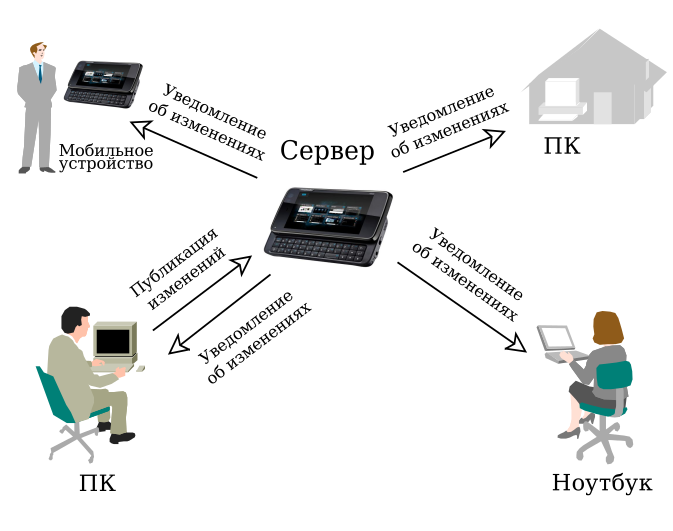
\includegraphics[width=\linewidth]{users_collaboration_example.pdf}
  \caption{Взаимодействие клиентов и сервера}
  \label{img:users_collaboration_example}
\end{figure} 

Подводя итог всему вышеперечисленному, был сформирован список требований к
выбираемой технологии промежуточного слоя.
\begin{itemize}
\item Взаимодействие основанное на клиент-серверной модели.
\item Не должно быть сложностей в создании сервера.
\item Сервер должен иметь возможность уведомления всех участников
взаимодействия.
\item Технология должна хорошо работать в условиях медленного, ненадежного
соединения с сетью Интернет, расположенного за NAT, прокси-сервером или
фаерволом.
\end{itemize}

Протокол XMPP c расширением публикации/подписки полностью удовлетворяет
вышеназванным требованиям и позволяет избежать почти все сложности, связанные с
реализацией клиент-серверной архитектуры, 

\subsection{Преимущества протокола XMPP}
XMPP (Extensible Messaging and Presence Protocol) "--- расширяемый протокол для
обмена сообщениями, в режиме близком к режиму реального времени. Протокол XMPP
может быть рассмотрен на нескольких уровнях абстракции. На нижнем уровне
абстракции, существует клиентское приложение, использующее протокол XMPP,
которое подключается к серверу и обменивается с ним сообщениями. Соединение с
сервером может быть установлено несколькими способами, даже поверх протокола
HTTP. На высоком уровне абстракции, клиент получает доступ ко всей XMPP сети,
где каждый её узел имеет уникальный идентификатор, называемый JID (Jabber
Identificator). Преимуществом протокола XMPP является то, что пересылка
сообщений между узлами сети не требует дополнительных усилий. Клиент создаёт
сообщение, адресованное другому клиенту и посылает его на сервер, который
отвечает за все операции, связанные с доставкой данного сообщения.

Большое преимущество протокола XMPP "--- расширяемость. Он может быть расширен с
помощью расширяющих протоколов (XEP). XMPP является открытым протоколом и каждый
желающий может создать высокоуровневый протокол на его основе. Организация XMPP
Standards Foundation отвечает за процесс создания и поддержки данных протоколов.
Одно из подобных расширений называется XEP-0060 Publish-Subscribe
\cite{xep-0060}. Оно отвечает за то, как реализовывать сервис
публикации/подписки поверх протокола XMPP. Любой участник XMPP сети имеет
возможность создать сервис публикации/подписки.

XMPP был создан как протокол мгновенного обмена сообщениями, использующий XML
для формирования сообщений. XML создаёт большой объём служебной информациии, что
может потребовать широкой полосы Интернет соединения. В XMPP сети, сообщения
между клиентом и сервером могут быть сжаты с использованием XEP-0138 (Stream
Compression). Таким образом, протокол XMPP имеет механизм, позволяющий
использовать его в сетях с малой полосой пропускания.

В настоящее время существует множество общедоступных XMPP серверов
поддерживающих общение в чате. Участие в подобных чатах доступно с мобильных
устройств и не требует широкополосного доступа в Интернет. С технической точки
зрения, совместное редактирование диаграмм очень похоже на участие в чате из
чего следует, что объём трафика не будет сильно отличаться. Исключением является
устройство, являющееся сервером. Данному устройству будет необходим более
широкий канал до сети Интернет для взаимодействия со многими клиентами.

\subsection{Выбор библиотеки для работы с XMPP протоколом}
Следующей задачей является выбор библиотеки языка Python, поддерживающей работу
с XMPP протоколом. На сайте XMPP Foundation \cite{xmpp} есть список из восьми
библиотек поддерживающих XMPP. Некоторые библиотеки более не поддерживаются
(jabber.py), некоторые требуют использования более новых (2.6, 3.x) версий языка
Python, недоступных под платформой Maemo (pyxmpp), другие же являются
исследовательскими проектами и не предназначены для повсеместного использования
(SleekXMPP). Twisted "--- единственный инструмент для работы с XMPP протоколом,
доступный в репозитории Maemo.

Twisted "--- событийно-ориентированный сетевой фреймворк, поддерживающий
множество протоколов таких как: TCP, UDP, SSL/TLS, HTTP, XMPP, NNTP, IMAP, SSH,
IRC, FTP и множество других \cite{twisted}. Twisted не имеет встроенной
поддержки XEP-0060, но существует внешняя библиотека Wokkel \cite{wokkel},
поддерживающая данное расширение. Данная библиотека отсутствует в репозитории
Maemo. Для того, чтобы иметь возможность её использовать, было принято решение о
создании и поддержки пакета для платформы Maemo.

\section{Архитектура сетевой подсистемы}
\subsection{XMPP расширение публикации/подписки}
Расширение XEP-0060 использует шаблон проектирования <<публикация/подписка
(publish-subscribe)>>, являющийся более общим относительно шаблона <<наблюдатель
(observer)>>. Данный шаблон состоит в следующем: объект подписывается на
обновления от другого объекта и становится его подписчиком. После того, как
подписчик публикует информацию, уведомление о данном событии (с опубликованной
информацией или без) пересылается всем подписчикам. В общем случае,
взаимодействие между подписчиками контролируется сервером, который получает
запрос на публикацию и производит рассылку уведомлений всем подписчикам.

Сервер может поддерживать подписку на различные сущности. В терминах расширения
XEP-0060, данные сущности называются узлами (nodes). Каждый подобный узел имеет
собственный список подписчиков. Узлы также могут хранить историю всех
уведомлений и обеспечивать другие сервисы определённые стандартом. Данные
получаемые сервером и пересылаемые на него называются элементом (item).
Описанная система организации данных может быть ассоциирована с организацией
файловой системы, где узлы представляют директории, а элементы соотносятся как
файлы.

В терминах XMPP расширения публикации/подписки, процесс взаимодействия может
быть представлен следующим образом. Пользователь создаёт сервер с единственным
узлом для обмена и хранения сообщений. Другие участники подписываются на
обновления от созданного узла. Когда один из публикующих делает изменения, они
пересылаются на сервер, который уведомляет всех подписчиков о произошедшем
событии. Данные пересылаются, используя возможности элемента содержать в себе
полезную нагрузку. Учитывая характер процесса взаимодействия между сервером и
подписчикам, была начата разработка сетевой архитектуры приложения.

\subsection{Распространение изменений}
\label{sec:changeset_propagation}
Приложение HiveMind, как и любой хороший редактор, имеет возможности отмены и
повтора ранее отмененных действий. Данная функциональность реализована на основе
QUndoStack, который хранит всю историю выполненных команд. Каждое изменение на
диаграмме связей атомарно. Когда пользователь совершает изменение создаётся
QUndoCommand. В QUndoCommand хранится информация для выполнения команды и для её
отката. Таким образом, использование QUndoStack позволяет двигаться по всей
истории изменений. Для каждого типа данных команд были созданы функции
сериализации и десериализации в XML. Изменения сделанные на карте отправляются
на сервис в виде XML сериализованных сообщений и не сохраняются в стеке команд.
Команды добавляются в стек только если они пришли как уведомления от сервиса,
поэтому подписчик должен ждать ответа от сервера для того чтобы увидеть
выполненные изменения (см рис. ~\ref{img:changeset_propagation}).

\begin{figure}
  \centering
  \includegraphics[width=\linewidth]{changeset-propagation.pdf}
  \caption{Диаграмма распространения изменений}
  \label{img:changeset_propagation}
\end{figure}

Для того чтобы управлять асинхронным взаимодействием был реализован класс
NetworkController. Все команды поступают в сетевой контроллер. Если сетевое
взаимодействие неактивно, команда добавляется в стек команд. В противном
случае, данная команда будет сериализована и отправлена на сервис. Уведомления
пришедшие от сервиса десериализуются в команды, добавляются в стек команд и
выполняются.

Данные команды содержат в себе информацию лишь об изменившейся части диаграммы.
Подобное условие необходимо для того, чтобы уменьшить объём пересылаемых данных,
который в противном случае будет чрезмерно большим. Необходимо чтобы все
участники имели одинаковые копии диаграмм, иначе команда, являющаяся корректной
с точки зрения одного участника, не будет являться таковой для другого. Поэтому
встаёт вопрос о распространении исходной диаграммы и её синхронизации между
всеми участниками в процессе взаимодействия.

Проблема распространения диаграммы была решена следующим образом: первый элемент
в узле должен содержать в себе сериализованную диаграмму связей. Все остальные
элементы содержат в себе сериализованные команды изменений. В момент, когда
человек становится подписчиком, ему пересылаются все элементы содержащиеся в
узле, включая диаграмму и совершенные ранее изменения.

Синхронизация диаграммы связей между всеми участниками представляет более
сложную проблему. Фактически речь идёт о сохранение целостности диаграммы связей
на сервере, то есть о контроле поступающих изменений. При поступлении
некорректного изменения, сервер должен его отбросить или провести слияние, если
возможно. К примеру, из-за задержек в соединении, пользователь может изменить
узел, который к этому времени уже был удалён одним из участников. В таком случае
сервер отсылает пользователю уведомление об ошибке и отбрасывает некорректное
изменение.

Подписчик может запросить все данные или часть данных, хранящихся в узле, в
любой момент времени. Данная возможность используется для синхронизации
локальной копии диаграммы с копией на сервере. К примеру, если изменение было
отброшено сервером, то подписчик производит синхронизацию своей диаграммы с её
версией на сервере. Сервер не нуждается в дополнительных способах синхронизации
диаграммы, поскольку все изменения локальны и всегда являются актуальными и
корректными.

\section{Реализация сетевой подсистемы}
Сетевая подсистема приложения была реализована поверх фреймворка Twisted и
библиотеки Wokkel. Wokkel является надстройкой над Twisted, добавляющей
фреймворку дополнительную функциональность. В частности Wokkel предоставляет
средства для более удобной реализации XMPP расширений (XEP) и имеет поддержку
следующих: Service Discovery (XEP-0030), Publish-Subscribe (XEP-0060).
Реализация расширения публикации/подписки в Wokkel не содержит бизнес-логики.
Это значит, что он отвечает за приём, генерацию и отправку сообщений в
соответствии со спецификацией XEP-0060. Wokkel реагирует на события, относящиеся
к публикации/подписке, делает разбор пришедших сообщений и вызывает
соответствующие обработчики.

Расширение публикации/подписки является одним из самых больших и сложных
стандартов XMPP. Реализация необходимого функционала, корректная с точки зрения
стандарта, могла занять большое количество времени. Поэтому было принято решение
использовать библиотеку Idavoll. Данная библиотека реализована на базе Wokkel и
реализует функциональность XEP-0060 необходимую для приложения, такую как:
<<Подписка>>, <<Публикация>>, <<Создание узлов>>, <<Хранилище элементов>>.
Библиотека Idavoll имеет хорошую архитектуру, позволяющую добавлять реализацию
новой функциональности, определенной стандартом расширения публикации/подписки.
Idavoll имеет множество классов необходимых для реализации стандарта XEP-0060
(см. рис. ~\ref{img:network_classes}).

Класс Node является абстрактным классом и представляют собой узел в терминах
XEP-0060. Существуют два типа узлов: LeafNode и CollectionNode. LeafNode может
содержать только элементы, когда как CollectionNode может содержать лишь другие
узлы. LeafNode хранит элементы в виде простого списка, но это не является
подходящим решением для приложения HiveMind. Как было сказано в главе
~\ref{sec:changeset_propagation}, необходимо проверять приходящие изменения на
корректность. Для этого был создан класс Changeset, хранящий в себе информацию о
самом изменении, его типе, времени создания и авторе данного изменения. Также
создан специальный класс-контейнер СhangesetStack, хранящий экземпляры класса
Changeset и отвечающий за корректность и согласованность изменений находящихся в
нём. HivemindNode унаследован от LeafNode и в отличии от него хранит изменения в
ChangesetStack.

\begin{figure}
  \centering
  \includegraphics[width=\linewidth]{idavoll-classes.pdf}
  \caption{Диаграмма сетевых классов}
  \label{img:network_classes}
\end{figure}

BackendService содержит реализацию бизнес-логики XEP-0060. В нем содержится
логика для работы с подписчиками, проверка прав доступа и т.д. Он связан
отношением композиции с классом Storage, отвечающим за управление узлами
(создание, удаление, конфигурирование). Класс HivemindNode, создаётся классом
Storage и содержит в себе методы для добавления данных, изменения конфигурации
узла, списка подписчиков и их ролей. PubSubService является классом библиотеки
Wokkel, отвечающим за разбор пришедших сообщений и вызов соответствующих
обработчиков. Если он содержит в себе экземпляр класса
PubSubResourceFromBackend, то помимо вызова своих обработчиков, осуществляется
передача уже разобранных сообщений в подходящие методы класса
PubSubResourceFromBackend. Этот классиспользования является дополнительным
уровнем абстракции, что позволяет делать архитектуру более гибкой.
PubSubResourceFromBackend обязательно содержит экземпляр класса BackendService,
которому он делегирует реализацию бизнес-логики.

Мобильные устройства зачастую имеют нестабильное соединение с сетью Интернет,
поэтому приложение должно иметь механизм, позволяющий обнаружить, что соединение
потеряно и уведомить об этом пользователя. Механизм проверки осуществляется
посредством XMPP Ping (XEP-0199) \cite{xep-0199}. Класс Pinger
ответственен за отсылку пинг сообщений и приём ответов. Проверка осуществляется
следующим образом: данный класс непрерывно отсылает пинг сообщения на XMPP
сервер, к которому подключен пользователь, если достигнуто определенное
количество пинг сообщений, оставшихся без ответа, то соединение рассматривается
как потерянное.

Похожий механизм используется для проверки статуса подписчиков. Каждый подписчик
имеет свой экземпляр класса Pinger, который отвечает за отсылку пинг сообщений
именно ему. На клиентской стороне реализован обработчик, который отвечает на
приходящие пинг сообщения от сервера приложения. Подписчиков может быть очень
много, поэтому был создан класс PingManager, отвечающий за управление
экземплярами класса Pinger (см. рис. ~\ref{img:ping_manager}). Он создаёт и
удаляет экземпляры класса Pinger, а также запускает или останавливает отправку
пинг сообщений до адресата. Pinger уведомляет NetworkController о состоянии
соединения с XMPP сервером, а также со всеми подписчиками. Пользователь может
увидеть статус соединения с подписчиками в диалоге редактирования прав
доступа(см. рис. ~\ref{img:permissions_dialog})

\begin{figure}
  \centering
  \includegraphics[scale=1.2]{ping-manager.pdf}
  \caption{Диаграмма классов, отвечающих за проверку состояния соединений}
  \label{img:ping_manager}
\end{figure}


\section{Система контроля доступа}
По умолчанию, все участники совместной работы имеют одинаковый доступ к
редактированию диаграммы связей. Такое поведение является подходящим для
случаев, когда необходимо создать множество идей или найти решение сложной
проблемы. Но существуют сценарии совместной работы, описанные в пункте ~\ref
{sec:collaborative_mindmapping}, при которых необходимо ограничить права доступа
некоторых пользователей. Для того, чтобы была возможность взаимодействия по
подобным сценариям, в HiveMind была реализована система контроля доступа.

Стандарт XEP-0060 заложена функциональность называемая моделью доступа (access
model), которая может быть сопоставлена с системой аутентификации. Пользователь,
открывающий доступ к диаграмме, может установить уровень доверия для новых
участников. Это значит, что пользователь может ограничить круг лиц, имеющих
право на присоединение к совместной работе. Было реализовано четыре модели
доступа:
\begin{itemize}
\item <<Открытая (open)>> --- поведение по умолчанию,  любой может
присоединиться;
\item <<Контакт лист (roster)>> --- только лица, находящиеся в контакт листе
владельца сервера имеют право на участие;
\item <<Интерактивная (authorize)>> --- владелец может выбирать тех, кто имеет
право на участие в совместной работе. Когда очередной человек подключается к
диаграмме, владелец получает запрос на присоединение;
\item <<Белый список (whitelist)>> --- новый участник может присоединиться, лишь
в том случае, если он находится в белом списке владельца сервера.
\end{itemize}

Следующая часть системы контроля доступа также заложена в стандарт XEP-0060 и
называется affiliations. Данная функциональность отвечает за авторизацию
пользователей. Каждый участник, присоединившийся к диаграмме, имеет свою роль,
определяющую набор допустимых действий. Было реализовано четыре роли:
\begin{itemize}
\item <<Изгнанник(outcast)>> --- не имеет права присоединяться и участвовать в
совместной работе;
\item <<Участник(member)>> --- имеет право только получать данные;
\item <<Издатель(publisher)>> --- имеет право получать и публиковать данные;
\item <<Владелец(owner)>> ---  имеет права издателя и может дополнительно
конфигурировать все аспекты сетевого взаимодействия.
\end{itemize}
Владелец сервера может в любой момент изменить роль человека, используя диалог
управления правами доступа (см. рис. ~\ref{img:permissions_dialog}).

\begin{figure}[b] 
  \centering
  \includegraphics[width=0.5\linewidth]{permissions_dialog.png}
  \caption{Диалог управления правами доступа}
  \label{img:permissions_dialog}
\end{figure}

XEP-0060 предоставляет возможность сделать систему контроля доступа еще более
гибкой. В некоторых случаях, может возникнуть необходимость временно позволить
всем участникам редактировать диаграмму. Для этого можно изменить роли всех
участников на издателя, что в случае большого количества участников является
утомительным и долгим занятием. Выходом из данной ситуации является реализация
функциональности называемой моделью публикации (publish model), определенной
стандартом XEP-0060. Данный механизм определяет, кто имеет право вносить
изменения на диаграмму связей. Было реализовано две модели публикации. Первый
тип модели позволяет вносит изменения участникам, имеющим роль издателя или
владельца. Во втором случае, все присоединившиеся участники имеют право на
внесение изменений.

Реализация системы контроля доступа позволила значительно увеличить количество
сценариев совместного взаимодействия. Данная система может быть улучшена, чтобы
увеличить количество областей применения приложения. Одной из подобных областей
является проведение презентаций, а точнее взаимодействие докладчика и
слушателей. В пункте ~\ref{sec:collaborative_mindmapping} был представлен
сценарий проведения презентации. Данный сценарий может расширен следующим
образом: позволить слушателям добавлять свои вопросы и пожелания на диаграмму
докладчика. В таком случае, необходимо, чтобы слушатели не могли изменять узлы
созданные докладчиком или другими слушателями, за что и будет отвечать
усовершенствованная система контроля доступа.

\newpage

\chapter*{Заключение}

\addcontentsline{toc}{chapter}{Заключение}

In this paper we proposed network subsystem architecture for collaborative mind
mapping based on the XMPP pubsub extension protocol. Our approach was
successfully implemented in HiveMind application, which allows teamwork mode on
various platforms including Maemo, MeeGo Netbook, and GNU/Linux.

HiveMind application can be downloaded from the project homepage at the
following URL: \emph{http://linuxlab.corp7.uniyar.ac.ru/projects/hivemind}. The
source codes are available from the Mercurial repository at
\emph{http://linuxlab.corp7.uniyar.ac.ru/hgpub/hivemind}.

The implemented network subsystem operates in terms of abstract commands, which
makes it loosely coupled from the application domain. It also makes possible to
spread our teamwork architecture to a broader class of applications which could
benefit from collaborative document editing.

Another direction for future development of the project is integration with
SmartConference System. This kind of work is in progress now.
\addto\captionsrussian{\def\bibname{Список литературы}}
\newpage
\addcontentsline{toc}{chapter}{Литература}
\begin{thebibliography}{99}

\bibitem{hivemind-8th-fruct}
\textit {Vasilev, A.}
HiveMind: Cross-platform Application for Collaborative Mind Mapping
/ A. Vasilev, A. Golovchenko, A. Kulikov, I. Paramonov
"--- Proceedings of the 8th Conference of Open Innovation Framework Program
FRUCT, 2010.
"---  219--224~с.

\bibitem{qt4}
\textit {Бланшет, Ж.} Qt 4. Программирование GUI на С++
/ Жасмин Бланшет, Марк Саммерфилд.
"--- КУДИЦ-Пресс, 2007.
"--- 648~с.

\bibitem{python}
\textit {Лутц, М.} Изучаем Python
/ М. Лутц
"--- Символ-плюс, 2009.
"--- 848~с.

\bibitem{pyqt4}
\textit {Summerfield, M.} Rapid GUI programming with Python and Qt : the
definitive guide to PyQt programming
/ M. Summerfield.
"--- Prentice Hall, 2007.
"--- 643~с.

\end{thebibliography}
\appendix

\makeatletter
\gdef\thechapter{\@Asbuk\c@chapter}
\makeatother

\chapter{Глоссарий}
\label{glossary}
Репозиторий "--- это место в файловой системе, управляемое системой контроля
версий, в которой хранятся исходные коды приложения и различные документы
вместе с историей их изменения и другой служебной информацией.

Вики-страница "--- это страница на сайте, содержимое которой пользователи могут
самостоятельно изменять с помощью инструментов предоставляемых сайтом.
Форматирование текста на таких страницах производится использованием
вики-разметки.

Метапрограммирование "--- это процесс написание компьютерных программ,
способных создавать и изменять другие программы или самих себя на этапе
компиляции или во время выполнения.

Ruby "--- динамический язык, который предоставляет широкие возможности для
метапрограммирования.

Модуль "--- Часть кода, выделенная специальным образом и
содержащая набор методов и констант.

Хук (Hook)"--- это программный интерфейс, который позволяет расширить
функциональность Redmine. При помощи Hook'a автор плагина имеет возможность
зарегистрировать функции обратного вызова, которые будут вызваны одна за
другой, при достижении участка кода, в котором расположен Hook.

Helper "--- это вспомогательный метод, позволяющий выделить
повторяющийся код в методы и получить преимущества от его многократного
использования.

Дерево DOM "---  это не зависящий от платформы и языка программный интерфейс,
позволяющий программам и скриптам получить доступ к содержимому HTML, XHTML и
XML-документов, а также изменять содержимое, структуру и оформление таких
документов.

Cron "--- это планировщик задач в UNIX-подобных операционных системах,
использующийся для периодического выполнения заданий в определённое время.
Регулярные действия описываются инструкциями, в конфигурационном файле.

Rake "--- это инструмент для автоматизации сборки программного кода,
использующий DSL на Ruby для определения различных задач.


\chapter{Исходные тексты расширений}

\section{Патч ensure-that-calendar-is-visible.patch}
\label{appendix:ensure-that-calendar-is-visible.patch}
\lstset{language={diff}}
\begin{lstlisting}
diff --git a/public/javascripts/calendar/calendar-setup.js b/public/javascripts/calendar/calendar-setup.js
--- a/public/javascripts/calendar/calendar-setup.js
+++ b/public/javascripts/calendar/calendar-setup.js
@@ -193,6 +193,18 @@
      cal.showAtElement(params.button || params.displayArea || params.inputField);
    else
      cal.showAt(params.position[0], params.position[1]);
+
+        var elementOffsets = $(cal.element).cumulativeOffset();
+        new Effect.Parallel(
+        [
+            new Effect.Tween(null, document.viewport.getScrollOffsets().top, elementOffsets[1], {sync: true},
+                function(p){ scrollTo(document.viewport.getScrollOffsets().left, p.round());}),
+            new Effect.Tween(null, document.viewport.getScrollOffsets().left, elementOffsets[0], {sync: true},
+                function(p){ scrollTo(p.round(), document.viewport.getScrollOffsets().top);})
+        ],
+        {duration: 1}
+        );
+
    return false;
  };
\end{lstlisting}

%%% Local Variables: 
%%% mode: latex
%%% TeX-PDF-mode: t
%%% TeX-master: "diploma"
%%% End: 

\end{document}
